
\documentclass[preprint,12pt]{elsarticle}

\usepackage[spanish]{babel}
\usepackage{amssymb}
\usepackage{graphicx}
\usepackage{lineno}
\usepackage[utf8]{inputenc}
\usepackage{url}
\usepackage{color}
\usepackage{enumerate} 
\usepackage[hidelinks]{hyperref}


\begin{document}
	
	\begin{frontmatter}
		
		
		\title{\huge DataWarehouse vs  Datalake}
		
		\author{Mamani Ayala, Brandon        (2015052715)}
		\author{Quispe Mamani, Angelo	      (2015052826)}
		\author{Vizcarra Llanque, Jhordy	      (2015052719)}
		\author{Ordoñez Quilli, Ronald          (2015052821)}
		\author{Rodriguez Mamani, Juan      (2017057862)}
		
		\address{Tacna, Perú}
		
		\begin{abstract}
			%% Text of we
			
The data warehouses in English take each importance day, as organizations move from schemes of only data collection to schemes of analysis of the same. However, in spite of the great diffusion of the concepts related to data warehouses, there is not too much Information available in Spanish regarding the methodologies fo implement them In this short article we will try to provide a general explanation of one of the most used methodologies. 
		\end{abstract}
\end{frontmatter}
%%

	
	%%
	%\linenumbers
	
	%% main text
	\section{Resumen}
Los almacenes de datos (data warehouses en inglés) toman cada día mayor importancia, a medida que las organizaciones pasan de esquemas de sólo recolección de datos a esquemas de análisis de los mismos. Sin embargo a pesar de la gran difusión de los conceptos relacionados con los almacenes de datos, no existe demasiada información disponible en castellano en cuanto a las metodologías para implementarlos. En este breve artículo intentaremos brindar una explicación general de una de las metodologías más usadas \\
	%%
	
	%%
	%\linenumbers
	
	%% main text



	%%
	
	%%
	%\linenumbers
	
	%% main text
\section{Introduccion}
\section{DataWarehouse}

Definición de Bill Inmon\\
\\Fue uno de los primeros autores en escribir sobre el tema de los almacenes de datos, define un data warehouse (almacén de datos) en términos de las características del repositorio de datos:

\begin{itemize}
	\item Orientado a temas: Los datos en la base de datos están organizados de manera que todos los elementos de datos relativos al mismo evento u objeto del mundo real queden unidos entre sí.
	\item Variante en el tiempo: Los cambios producidos en los datos a lo largo del tiempo quedan registrados para que los informes que se puedan generar reflejen esas variaciones.
	\item No volátil: La información no se modifica ni se elimina, una vez almacenado un dato, éste se convierte en información de sólo lectura, y se mantiene para futuras consultas.
	\item Integrado: La base de datos contiene los datos de todos los sistemas operacionales de la organización, y dichos datos deben ser consistentes.
\end{itemize}

Definición de Ralph Kimball\\
\\Define un almacén de datos como: "Es un almacén de datos que extrae, limpia, conforma y entrega una fuente de datos dimensional para la consulta y el análisis". También fue Kimball quien determinó que un data warehouse no era más que: "la unión de todos los Data marts de una entidad". Defiende por tanto una metodología ascendente (bottom-up) a la hora de diseñar un almacén de datos.


\subsection{Materiales y Metodos}

ESTRUCTURA\\
\\La arquitectura de un data warehouse puede ser dividida en tres estructuras simplificadas: básica, básica con un área de ensayo y básica con área de ensayo y data marts.

\begin{itemize}
	\item Con una estructura básica, sistemas operativos y archivos planos proporcionan datos en bruto que se almacenan junto con metadatos. Los usuarios finales pueden acceder a ellos para su análisis, generación de informes y minería.
	\item Al añadir un área de ensayo que se puede colocar entre las fuentes de datos y el almacén, ésta proporciona un lugar donde los datos se pueden limpiar antes de entrar en el almacén. Es posible personalizar la arquitectura del almacén para diferentes grupos dentro de la organización.
	\item Se puede hacer agregando data marts, que son sistemas diseñados para una línea de negocio en particular. Se pueden tener data marts separados para ventas, inventario y compras, por ejemplo, y los usuarios finales pueden acceder a datos de uno o de todos los data marts del departamento.
\end{itemize}

\begin{center}
	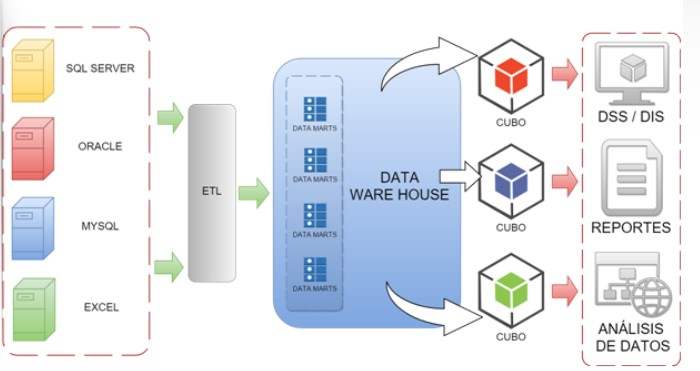
\includegraphics[width=12cm]{./Imagenes/imagen1} 
\end{center}

ETL (Extract-Transform-Load)\\
\begin{itemize}
	\item Extracción: obtención de información de las distintas fuentes tanto internas como externas.
	\item Transformación: filtrado, limpieza, depuración, homogenización y depuración de la información.

\begin{center}
	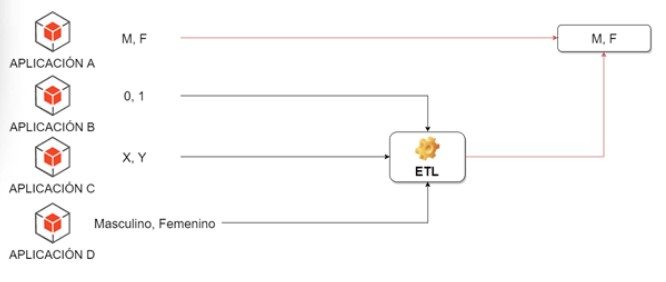
\includegraphics[width=12cm]{./Imagenes/imagen2} 
\end{center}

	\item Carga: Organización y actualización de los datos y los metadatos de la base de datos.
\end{itemize}

DATA MART\\
\\Es una base de datos departamental, especializada en un área de negocio especifica. Se caracteriza por disponer la estructura optima de datos para analizar el informacional detalle desde todas las perspectivas que afecten a los procesos de dicho negocio.

\begin{center}
	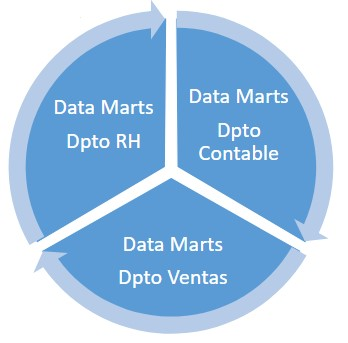
\includegraphics[width=6cm]{./Imagenes/imagen3} 
\end{center}

CUBOS\\
\\Es una base de datos especial, en la cual el almacenamiento físico de los datos se realiza en un vector multidimensional.
\begin{center}
	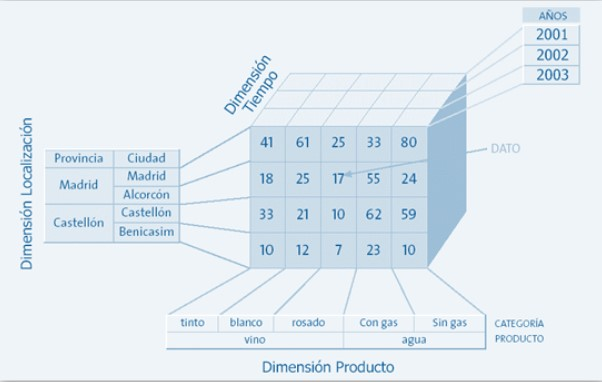
\includegraphics[width=12cm]{./Imagenes/imagen4} 
\end{center}


\subsection{Modos de Uso del Data WareHouse}
\begin{itemize}
	\item Para tener un mayor conocimiento del negocio
	\item Para tomar mejores decisiones y en un tiempo menor.
	\item Para mejorar y ser más efectivos.
	\item Para no perder distancia con la competencia.
\end{itemize}
 Las data warehouse son la base para los sistemas de gestión de relaciones con los clientes, ya que pueden ser utilizados para la consolidación de los datos del cliente y la identificación de áreas de satisfacción y/o frustración del cliente.
\\
También se utilizan para la detección de fraudes, análisis de reposicionamiento de producto, el descubrimiento de centros de beneficio y gestión de activos corporativos. 
\\\\Ejemplos:
\begin{itemize}
	\item Para los minoristas, un almacén de datos o data warehouse puede ayudar a identificar las características demográficas de los clientes, identificar los patrones de compra y mejorar las respuestas de correo directo. 
	\item Para los bancos, puede ayudar en la detección de fraude de tarjetas de crédito, ayudar a identificar a los clientes más rentables, y poner de relieve los clientes más fieles.
	
\end{itemize}

\subsection{Data Lake vs Data Warehouse}
\begin{itemize}
	\item Un Data Lake conserva todos los datos, a diferencia del almacen de datos, donde se dedica una parte importante de tiempo a decidir quq datos incluir y no incluir en el almacen.
\item Un Data Lake admite todos los tipos de datos, independientemente de su tipo, formato o procedencia y sin necesidad de normalizar su estructura. La información se mantiene en su forma original y solo se transforma cuando se va a consumir.
	\item El Data Lake puede nutrir a todos los usuarios de la organización, incluyendo a esos perfiles técnicos con exigencias de análisis más avanzadas, que son quienes recurren a capacidades como análisis estadístico y modelado predictivo.
	\item A diferencia del Data Warehouse, el Data Lakes se adapta fácilmente a los cambios. El diseño del almacén es un proceso complejo y, la actualidad de los negocios, en ocasiones no puede esperar tanto tiempo. Para esas circunstancias, asegura la adaptabilidad necesaria para entregar respuestas más rápidas.
	
\end{itemize}
\subsection{Herramientas para Implementar un Data Warehouse}

-Productos Comerciales
\begin{itemize}
	\item Atlas SBI
	\item Bitool Herramienta de ETL y Visualizacion
	\item Bingo Intelligence
	\item BIRT Analytics	
	\item Business Objects	
	\item Dynamic Data Web	
\end{itemize}
-Productos Open Source
\begin{itemize}
	\item SpagoBI
	\item Pentaho
	\item OpenI: Aplicación Web simple orientada al reporting OLAP.
	\item LogiReport: Aplicación de BI gratuita basada en Web de LogiXML	
	\item JasperReports	
	\item Eclipse BIRT Project: Generador de informes para aplicaciones Web de código abierto basado en Eclipse	
\end{itemize}
\subsection{Conclusiones}
\begin{itemize}
	\item Las particiones no se procesaban en paralelo si no secuencialmente, lo que hace que sea más lento el procesamiento.
	\item No se pueden usar multiples idiomas.
	\item Si son muchos datos tarda bastante en manejar configuraciones de diferentes particiones.
	\item El modelo tabular acapara demasiada memoria RAM y a su vez es dependiente de tal que afectará a otras aplicaciones.
\end{itemize}

\section{Datalake}

Un data lake es un repositorio de almacenamiento que contienen una gran cantidad de datos en bruto y que se mantienen allí hasta que sea necesario. A diferencia de un data warehouse jerárquico que almacena datos en ficheros o carpetas, un data lake utiliza una arquitectura plana para almacenar los datos.\\

A cada elemento de un data lake se le asigna un identificador único y se etiqueta con un conjunto de etiquetas de metadatos extendidas. Cuando se presenta una cuestión de negocios que debe ser resuelta, podemos solicitarle al data lake los datos que estén relacionados con esa cuestión. Una vez obtenidos podemos analizar ese conjunto de datos más pequeño para ayudar a obtener una respuesta.\\

El data lake se asocia a menudo con el almacenamiento de objetos orientado a Hadoop. En este escenario, los datos de una organización se cargan primero en la plataforma Hadoop y, a continuación, se aplican las herramientas de análisis y de minería de datos a los datos que residen en los nodos clúster de Hadoop. \\

\subsection{Beneficios}
\begin{itemize}
\item El principal beneficio de un data lake es la centralización de fuentes de contenido dispares. Una vez reunidas (de sus "silos de información"), estas fuentes pueden ser combinadas y procesadas utilizando big data, búsquedas y análisis que de otro modo hubieran sido imposibles. Las fuentes de contenido dispares a menudo contienen información confidencial que requerirá la implementación de las medidas de seguridad apropiadas \\
\item Es posible que algunos usuarios no necesiten trabajar con los datos en el origen de contenido original, sino consumir los datos resultantes de los procesos incorporados a dichos orígenes. Puede haber un límite de licencias para el origen de contenido original que impide que algunos usuarios obtengan sus propias credenciales. En algunos casos, la fuente de contenido original se ha bloqueado, está obsoleta o se desactivará en breve, sin embargo, su contenido sigue siendo valioso para los usuarios del data lake.\\
\item Es posible que algunos usuarios no necesiten trabajar con los datos en el origen de contenido original, sino consumir los datos resultantes de los procesos incorporados a dichos orígenes. Puede haber un límite de licencias para el origen de contenido original que impide que algunos usuarios obtengan sus propias credenciales. En algunos casos, la fuente de contenido original se ha bloqueado, está obsoleta o se desactivará en breve, sin embargo, su contenido sigue siendo valioso para los usuarios del data lake.\\
\item Una vez que el contenido está en el data lake, puede normalizarse y enriquecerse. Esto puede incluir extracción de metadatos, conversión de formatos, aumento, extracción de entidades, reticulación, agregación, des-normalización o indexación.\\
\item Los datos se preparan "según sea necesario", lo que reduce los costos de preparación sobre el procesamiento inicial (tal como sería requerido por los data warehouses. Una estructura de big data permite escalar este procesamiento para incluir los conjuntos de datos más grandes posibles.\\
\item Los usuarios, de diferentes departamentos, potencialmente dispersos por todo el mundo, pueden tener acceso flexible a un data lake y a su contenido desde cualquier lugar. Esto aumenta la reutilización del contenido y ayuda a la organización a recopilar más fácilmente los datos necesarios para impulsar las decisiones empresariales.\\
\item La información es poder, y un data lake pone la información de toda la empresa en manos de muchos más empleados para hacer a la organización un todo más inteligente, más ágil y más innovadora.
\end{itemize}
\subsection{Principales Diferencias entre DataLakes y Data Warehouses}

\subsubsection{Una Data Lake conserva todos los datos}

Durante el desarrollo de un data warehouse, se gasta una cantidad considerable de tiempo analizando las fuentes de datos, entendiendo los procesos de negocio y perfilando los datos. El resultado es un modelo de datos altamente estructurado diseñado para la generación de informes. Una gran parte de este proceso incluye tomar decisiones sobre qué datos incluir y no incluir en el almacén. Generalmente, si los datos no se utilizan para responder a preguntas específicas o en un informe definido, pueden excluirse del almacén. Esto se hace generalmente para simplificar el modelo de datos y también para conservar el costoso espacio en el almacenamiento de disco que se utiliza para hacer el data warehouse.\\

En contraste, el data lake conserva todos los datos. No sólo los datos que se utilizan actualmente, sino los datos que se pueden utilizar e incluso los datos que nunca se van a ser utilizados sólo porque quizás podrían ser utilizados algún día. Los datos también se mantienen todo el tiempo para que podamos volver en el tiempo a cualquier punto para hacer el análisis.\\

Este enfoque se hace posible porque el hardware para un data lake suele ser muy diferente del utilizado para un data warehouse. La ampliación de un data lake a terabytes y petabytes puede hacerse de manera bastante económica.\\

\subsubsection{Un Data Lake soporta todos los tipos de datos}

Los data warehouses generalmente se componen de datos extraídos de sistemas transaccionales junto con métricas cuantitativas y los atributos que las describen. Las fuentes de datos no tradicionales, como los registros del servidor web, los datos de sensores, la actividad de las redes sociales, el texto y las imágenes, se ignoran en gran medida. Se siguen encontrando nuevos usos para estos tipos de datos, pero consumirlos y almacenarlos puede ser costoso y difícil.\\

El enfoque del data lake abarca estos tipos de datos no tradicionales. En el data lake, guardamos todos los datos independientemente de la fuente y la estructura. Los mantenemos en su forma bruta y sólo los transformamos cuando estamos listos para usarlos. Este enfoque se conoce como "Schema on Read" en comparación con el "Schema on Write" que es el enfoque utilizado en el data warehouse.\\

\subsubsection{Un Data Lakes soporta a todos los usuarios}

En la mayoría de las organizaciones, el 80 Porcieno o más de los usuarios son "operacionales". Quieren obtener sus informes, ver sus KPIs o seleccionar el mismo conjunto de datos en una hoja de cálculo todos los días. El data warehouse suele ser ideal para estos usuarios porque está bien estructurado, fácil de usar y comprender y está diseñado para responder a sus preguntas.\\

El siguiente 10 Porciento más o menos, hace más análisis en esos datos. Utilizan el data warehouse como una fuente, pero a menudo vuelven a los sistemas de origen para obtener datos que no están incluidos en el almacén y a veces traen datos de fuera de la organización. Su herramienta favorita es la hoja de cálculo y crean nuevos informes que a menudo se distribuyen en toda la organización. El data warehouse es su fuente de acceso a los datos, pero a menudo van más allá de sus límites\\

Por último, el restante tanto por ciento de los usuarios hace un análisis profundo. Pueden crear fuentes de datos totalmente nuevas basadas en la investigación. Ellos mezclan muchos tipos diferentes de datos y llegan a nuevas preguntas que deben responderse. Estos usuarios pueden utilizar el data warehouse, pero a menudo lo ignoran, ya que normalmente se les solicita que vayan más allá de sus capacidades. Estos usuarios incluyen a los científicos de datos y pueden utilizar avanzadas herramientas analíticas y capacidades como el análisis estadístico y el modelado predictivo.\\

El enfoque del data lake soporta igualmente a todos estos usuarios. Los científicos de datos pueden ir al data lake y trabajar con el gran y variado conjunto de datos que necesitan, mientras que otros usuarios hacen uso de vistas más estructuradas de los datos proporcionadas para su uso.\\

\subsubsection{Los Data Lakes se adaptan fácilmente a los cambios}

Una de las principales quejas sobre los data warehouses es cuánto tiempo se tarda en cambiarlos. Un tiempo considerable se gasta por adelantado durante el desarrollo de la estructura del almacén. Un buen diseño de almacén puede adaptarse al cambio, pero debido a la complejidad del proceso de carga de datos y al trabajo realizado para facilitar el análisis y la elaboración de informes, estos cambios necesariamente consumirán algunos recursos de desarrolladores y tomarán algún tiempo.\\

Muchas preguntas comerciales no pueden esperar a que el equipo del data warehouse adapte su sistema para responderlas. La necesidad cada vez mayor de respuestas más rápidas es lo que ha dado lugar al concepto de auto-servicio de inteligencia empresarial.\\

En el data lake, por otro lado, como todos los datos se almacenan en bruto y siempre con accesibles a alguien que necesite utilizarlos, los usuarios tienen el poder de ir más allá de la estructura del almacén para explorar datos de nuevas maneras y responder a sus preguntas a su ritmo.\\

Si se demuestra que el resultado de una exploración es útil y existe el deseo de repetirlo, entonces se puede aplicar un esquema más formal y se puede desarrollar la automatización y la reutilización para ayudar a extender los resultados a un público más amplio. Si se determina que el resultado no es útil, puede descartarse y no se han realizado cambios en las estructuras de datos ni se han consumido recursos de desarrollo.\\

\subsubsection{ Los Data Lakes proporcionan una visión más rápida}

Esta última diferencia es realmente el resultado de las otras cuatro. Debido a que los data lakes contienen todos los datos y tipos de datos, y a que permite a los usuarios acceder a los datos antes de que se hayan transformado, limpiado y estructurado, permite a los usuarios llegar a sus resultados más rápido que el método tradicional de data warehouse.\\

Sin embargo, este acceso temprano a los datos tiene un precio. El trabajo típicamente realizado por el equipo de desarrollo de data warehouse no se puede hacer para algunas o todas las fuentes de datos requeridas para realizar un análisis. Esto permite a los usuarios explorar y usar los datos como mejor les parezca, pero el primer nivel de usuarios de negocios que he descrito anteriormente tal vez no quiera hacer ese trabajo. Todavía quieren sus informes y KPI's.\\

En los data lakes, estos consumidores de informes operativos harán uso de vistas más estructuradas de los datos en el data lake que se parecen a lo que siempre han tenido antes en el data warehouse. La diferencia es que estas vistas existen principalmente como metadatos que se sitúan sobre los datos en el lago en lugar de tablas físicamente rígidas que requieren un desarrollador para cambiarlas.\\



\subsection{Materiales y Metodos}

\subsubsection{Supervicion arquitectonica}
	
Una vez que tienes la alineación del negocio y sabes cuáles son sus prioridades, necesitas definir la arquitectura inicial: ¿cuáles son los diversos componentes que necesitarás, y cómo será la plataforma técnica final? Ten en cuenta que se trata de una inversión a largo plazo, por lo que necesitas pensar cuidadosamente acerca de hacia dónde se está moviendo la tecnología. Naturalmente, es posible que no tengas todas las respuestas por adelantado, por lo que podría ser necesario realizar una prueba de concepto para obtener alguna experiencia y afinar y aprender a lo largo del camino. Un aspecto especialmente importante de tus planes arquitectónicos es una buena estrategia de gestión de datos que incluya el gobierno de datos y los metadatos, y cómo captará eso. Es crítico si se quiere construir un data lake administrado y gobernado en lugar del temido "pantano de datos". \\

\subsubsection{Estrategia de Seguridad}

Esboza una estrategia de seguridad robusta, especialmente si tu data lake va a ser una plataforma compartida utilizada por múltiples líneas de unidades de negocio o por partes interesadas tanto internas como externas. La privacidad y la seguridad de los datos son fundamentales, especialmente para los datos confidenciales. Puede que incluso tengas que incluir reglas regulatorias. También debes pensar en multiusuario: ciertos usuarios pueden no ser capaces de compartir datos con otros usuarios. Si se está sirviendo a varias audiencias externas, cada cliente puede tener acuerdos de datos individuales y deben respetarse.

\subsubsection{I/O y modelo de memoria}

Como parte de la plataforma tecnológica y su arquitectura, se debe pensar en lo que será las capacidades de escalar del data lake. Por ejemplo, ¿se va a usar el desacoplamiento entre el almacenamiento y las capas de computación? Si ese es el caso, ¿cuál es la capa de almacenamiento persistente? Se deben comprender a fondo los requisitos de rendimiento desde el punto de vista de la ingesta de datos, lo que determinará el rendimiento para el almacenamiento y la red, así como si se pueden procesar datos de manera oportuna.

\subsubsection{Plan de operaciones}

Piensa en el data lake desde una perspectiva de acuerdo de nivel de servicio (SLA): ¿qué requisitos de SLA esperan tus interlocutores empresariales?, especialmente en lo que se refiere a aplicaciones críticas para el negocio que afectan ingresos. Se necesitan SLAs adecuados en términos de tiempo de inactividad, y en términos de datos que son ingeridos, procesados y transformados de una manera repetible. Volviendo al punto de las personas y habilidades, es fundamental contar con las personas adecuadas con experiencia en la gestión de estos entornos, para formar un equipo de operaciones para apoyar los acuerdos de nivel de servicio y cumplir con los requisitos del negocio.

\subsubsection{Plan de comunicaciones}

Una vez que tengas el data lake en su sitio, ¿cómo se anunciará este hecho en la empresa y como traerás usuarios adicionales? Es necesario conseguir diferentes interesados de negocios y mostrar algunos éxitos para su entorno de data lake para prosperar. Como cualquier otra plataforma de TI, su éxito, en última instancia, se basa en su adopción por parte del negocio.

\subsubsection{Plan de comunicaciones}

Dependiendo de la criticidad de negocio de tu data lake y de los diferentes SLAs que tengas con los diferentes grupos de usuarios, necesitarás un plan de recuperación de desastres que pueda soportarlo.


\subsection{Data Lake Inteligente}

Las organizaciones buscan aprovechar las nuevas plataformas de procesamiento de datos, como Apache Hadoop, para poder llevar a cabo algunas ideas previas inaceptables. La aparición de Apache Hadoop y el concepto de data lake ofrece a las organizaciones el lujo de agrupar todos los datos para que sean accesibles por los usuarios en cualquier momento para cualquier tipo de análisis.\\

Las organizaciones recolectan datos de clientes y de mercado por su potencial para mejorar las experiencias e impulsar el crecimiento del negocio. Las instituciones financieras están ahorrando y monitorizando los datos transaccionales y otras señales relacionadas con el fin de enriquecer las técnicas de detección de fraude, mantenerse al día con las regulaciones globales cambiantes y aumentar la confianza del consumidor en la seguridad de sus servicios. Las organizaciones relacionadas con temas de salud están preservando los datos de registros médicos electrónicos y los datos de reclamaciones con el fin de impulsar un cuidado de la salud más personalizado. La oportunidad de aprovechar los datos nunca ha sido mayor que con la tecnología de big data.

\subsection{Resultados}

\subsection{Conclusiones}

\begin{itemize}
	\item Las particiones no se procesaban en paralelo si no secuencialmente, lo que hace que sea más lento el procesamiento.
	\item No se pueden usar multiples idiomas.
	\item Si son muchos datos tarda bastante en manejar configuraciones de diferentes particiones.
	\item El modelo tabular acapara demasiada memoria RAM y a su vez es dependiente de tal que afectará a otras aplicaciones.
\end{itemize}



%%
	
	%%
	%\linenumbers
	
	%% main text

	
	\newpage
	
		%ESTILO
	%ARCHIVO .bib
	   \begin{thebibliography}{0}
              \bibitem{Juan} https://bib.irb.hr/datoteka/102195.t09r02.pdf 
                 \bibitem{Juan} https://www.sarjen.com/2016/03/15/what-are-the-pros-and-cons-of-tabular-model-over-multi-dimension-cube-and-relation-database/
                 \bibitem{Juan} https://www.element61.be/en/resource/choice-between-tabular-or-multidimensional-models-sql-server-analysis-services-2012
                  \bibitem{Jhordy} https://docs.microsoft.com/es-es/sql/analysis-services/comparing-tabular-and-multidimensional-solutions-ssas?view=sql-server-2017
 \bibitem{Jhordy} https://www.businessintelligence.info/definiciones/que-es-modelo-dimensional.html
                    \bibitem{Brandon} https://www.businessintelligence.info/definiciones/que-es-modelo-dimensional.html


         \end{thebibliography}
	
\end{document}

%%
%% End of file `elsarticle-template-1-num.tex'.
